На пазара в момента съществува огромен потенциал за този тип приложения, тъй като бизнес моделът, който искаме да постигнем, е доказано ефективен. Пример за това е Airbnb, който в рамките на няколко години стана едно от най-успешните приложения, набавяйки си милиони потребители от целия свят. 

Разглеждайки съществуващи такива продукти на пазара откриваме, че има недостиг на възможности човек да намери битова работа, чрез която да си изкара пари. Всички съществуващи вече продукти страдат от лош бизнес модел и несигурна за потребителя система. 
\section{Съществуващи продукти с подобни цели}
\subsection{TaskRabbit}
TaskRabbit е уеб и мобилно приложение, което свързва фрийланс работници с локални работодатели, позволяващо на хората да намират незабавна помощ с битова работа като готвене, местене и доставки. TaskRabbit е най-известното приложение в тази сфера, но въпреки това страда от доста недостатъци.
\begin{figure}[h]
    \centering
   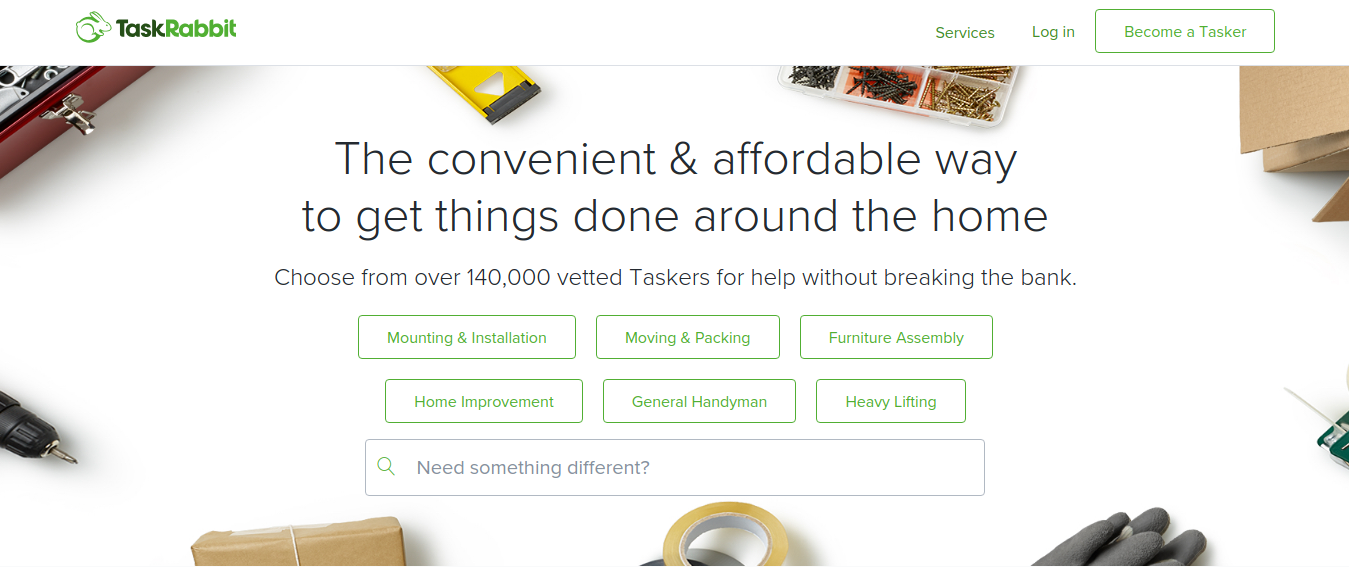
\includegraphics[scale=.3]{images/taskRabbitWeb.png}
    \caption{TaskRabbit - Титулна страница}
    \label{fig:taskRabbitWeb}
\end{figure}

Услугата не е достъпна за България и регистрирането е сложен процес, който изисква прекалено много време и струва пари. Приложението също не е достатъчно гъвкаво за различните типове работа. 

\subsection{Airbnb}

\begin{figure}[h]
    \centering
   
\includegraphics[scale=.3]{images/airbnb.png}
    \caption{Airbnb - Титулна страница}
    \label{fig:airbnb}
\end{figure}

Airbnb е услуга, която предлага наемането и даването под наем на апартаменти. Специалното за тяхната услуга е, че всеки може да даде под наем своя стая или апартамент, което позволява за повече гъвкавост и от двете страни на услугата. За наемащите спестява пари, тъй като цените на апартаменти и стаи са драстично по-ниски отколкото хотелски такива. За даващите под наем е лесен начин за изкарване на пари. Всеки, който има апартамент или стая, която не използва, може да си осигури доход чрез техните услуги. Airbnb бързо добива популярност поради иновацията и възможностите, които предоставя на клиентите си.

Причината да съм добавил Airbnb към този списък е поради общото между функционалността на тяхната услуга и нашата идея. Много от идеите на проекта са вдъхновени от техните услуги, тъй като и при тях трябва да се покрие размяната на сумите, осигуряването на връзката между клиентите и създаването на обявите.

\section{Развойни среди}
    \subsection{Eclipse}
    
    \begin{figure}[h]
        \centering
        
\includegraphics[scale=.2]{images/eclipse.jpg}
        \caption{Eclipse Лого}
        \label{fig:eclipse_logo}
    \end{figure}
    
    Eclipse е среда за разработване на софтуер, написана на Java. Използва плъгини за да предостави функционалност на различни езици. Възможно е да се пише на C, Python, както и езици като LaTeX за документиране. Дълго време тази среда бива основа в разработката на Java софтуер, но е изместен от IntelliJ, който разглеждаме във втора глава.

    \subsection{NetBeans}
    
    \begin{figure}[h]
        \centering
       
\includegraphics[scale=.05]{images/netbeans.png}
        \caption{Netbeans Лого}
        \label{fig:netbeans_logo}
    \end{figure}
    
    Netbeans е интегрирана среда за разработка, на която може да се пише на Java, JavaScript, PHP, Python, Ruby, Groovy, C, C++, Scala, Clojure и други езици. За удължаване на функционалността на средате, клиент може да инсталира модули създадени от трето лице изработчик.
    Средата е създадена с цел да предлага интелигентен и бърз начин за писане на код. За жалост обаче страда от по-малка общност отколкото Eclipse или IntelliJ, което ограничава възможността от плъгини, които могат да бъдат инсталирани.
    Netbeans има способността да работи на повечето съвременни операционни системи.
    
    \subsection{Maven}
    Maven е технология за автоматизиране на проектите като ги сглобява. Използва се основно за Java проекти.
    Тя покрива две части от компилирането на софтуер. Първата е \textbf{начинът}, по който се компилират и второто е как да се описват зависимостите на проект. Maven динамично изтегля пакети, които са дефинирани във файла му и ги изтегля през интернет, което улеснява процеса за играждане на цялостния продукт, елиминирайки нуждата от ръчно изтегляне на пакети и добавяне към проекта.
    
    \subsection{Gradle}
    Gradle е също технология за автоматизиране на проектите, но е по-ефективна, по-бърза и по-лесна за използване от Maven. За този проект именно нея съм предпочел от двете поради изброените причини. Всички фунцкионалности, които Maven предлага са покрити и от Gradle.
    
    \begin{figure}[h]
    \centering
    \makebox[\textwidth][c]{
\includegraphics[width=0.2\textwidth]{images/gradle.png}}%
    \caption{Gradle Лого}
    \label{fig:gradle}
\end{figure}


